\documentclass{inVerba-notes}

\newcommand{\theTitle}{\href{https://github.com/cullyn-inverba/notes/tree/master/bi-428} {Human Genetics}}

\begin{document}
\hypertarget{ToC}{\tableofcontents}

%%%%%%%%%%% DNA Structure and Function %%%%%%%%%%%
%\begingroup
\chapter{DNA Structure and Function}\label{DNA Structure and Function}
\begin{adjustwidth}{1cm}{1cm}
  This chapter was mostly basic review material. The portion on DNA was more of a test of my recent changed document class settings. The majority of the chapter was omitted. I might add more review content later if I find necessary.
\end{adjustwidth}

\section{Deoxyribonucleic Acid}\label{Deoxyribonucleic Acid}
\begin{itemize}
    \item \ddd{Deoxyribonucleic Acid (DNA)}: a double helix containing two polynucleotide chains that carries the genetic instructions for all known organisms and many viruses.
        \begin{itemize}
            \item The bases are made of four bases:
                \begin{itemize}
                    \item The \yyy{purine} derivatives: \yyy{adenine (A) and guanine (G)}.
                    \item The \xxx{pyrimidine} derivatives: \xxx{thymine (T) and cytosine (C)}.
                \end{itemize} 
            \item The backbone is made of \emph{alternating deoxyribose} molecules (a ribose missing its 2' oxygen) connected to phosphodiester bonds from \emph{5' \to\ 3'} positions---forming two \emph{antiparallel} strands.
            
                \centering
                \schemestart{}
                \chemname{\chemfig[cram width=2pt]{HO-[2,0.5,2]?<[7,0.7](-[6,0.5]OH)-[,,,,line width=2pt](-[6,0.5]\emph{OH})>[1,0.7](-[6,0.5]OH)-[3,0.7]O-[4]?}}{Ribose}
                \arrow{}
                \chemname{\chemfig[cram width=2pt]{HO-[2,0.5,2]?<[7,0.7](-[6,0.5]OH)-[,,,,line width=2pt](-[6,0.5]\emph{H})>[1,0.7](-[6,0.5]OH)-[3,0.7]O-[4]?}}{Deoxyribose}
                \schemestop{}
        \end{itemize}
    \item Number of \yyy{adenines} = \xxx{thymines}. (A-T)
    \item Number of \yyy{guanines} = \xxx{cytosines}. (C-G)
        \begin{itemize}
            \item Bonds between bases are \emph{noncovalent} (no electron sharing, weak).
            \item C---G pairs form three hydrogen bonds, while A---T forms two; making G---C slightly more stable.
            
            \scriptsize
            \yyy{\chemname%
            {\chemfig{@{H1}H-[:180]N(-[:-120]H)-[:120]*6(-N(-@{H2}H)-(=@{O3}O)-(*5(-N=-N(-R)-))=-N=)}}
            {\normalsize Guanine}}
          \qquad
          \xxx{\chemname%
            {\chemfig{@{O1}O=[:60]*6(-N(-R)-=-(-N(-[::60]@{H3}H)-[::-60]H)=@{N2}N-)}}
            {\normalsize Cytosine}}
          \chemmove[dashed]{\draw (H1)--(O1) (H2)--(N2) (O3)--(H3) ;}
          \hspace{18pt}
          \yyy{\chemname%
            {\chemfig{-[:120,,,,back]*6(-N(-@{H2}H)=(-NH-[:0]@{H4}H)-(*5(-N=-N(-R)-))=-N=)}}
            {\normalsize Adenine}}
          \qquad
          \xxx{\chemname%
            {\chemfig{O=[:60]*6(-N(-R)-=(-)-(=@{O}O)-@{N2}N-)}}
            {\normalsize Thymine}}
          \chemmove[dashed]{\draw (H2)--(N2) (H4)--(O) ;}
        \end{itemize} 
\end{itemize}
%\endgroup
%%%%%%%%%%% DNA Structure and Function %%%%%%%%%%%

%%%%%%%%%%% Genetic Variation %%%%%%%%%%%
%\begingroup
\chapter{Genetic Variation}\label{Genetic Variation}
\begin{adjustwidth}{1cm}{1cm}
  Much of this chapter was once again mostly review. However, the mini-section on nomenclature was new to me and seemed useful, so I included this. This chapter provided several hooks for related topics, so I may add more content from elsewhere in this chapter if I find my understanding on basic material lacking.
\end{adjustwidth}

\section{Mutation Nomenclature}\label{Mutation Nomenclature}
\begin{multicols}{2}
\begin{itemize}
  \item \textbf{Level of mutational change}:
    \begin{itemize}
      \item \emph{g} = Genomic
      \item \emph{c} = Coding sequence
      \item \emph{m} = Mitochondrial sequence
      \item \emph{r} = RNA sequence
      \item \emph{p} = Protein sequence
      \item \emph{E+I or E-I} = Explained below
    \end{itemize}
  \item \textbf{Type of mutational change}:
    \begin{itemize}
      \item \emph{>} = Substitution in the DNA
      \item \emph{\_} = A range of affected bases
      \item \emph{del} = Deletion
      \item \emph{dup} = Duplication
      \item \emph{ins} = Insertion
      \item \emph{inv} = Inversion
    \end{itemize}
  \end{itemize}
  \end{multicols}
  \begin{itemize}
    \item \emph{E+I} = The last nucleotide of preceding exon (E) for genomic mutations at the 5' (+) and number of nucleotides into the intron (I).
    \item \emph{E-I} = The first nucleotide of the next exon (E) for mutations at the 3' end of an intron (-) and the number of nucleotides into the intron (I).
  \subsection{Nomenclature Examples}
  \begin{itemize}
      \item \emph{g.1346A>C}: Change of A to C at position 1346 in the genomic DNA sequence.
      \item \emph{c.745delT}: Deletion of T at position 745 in the coding sequence.
      \item \emph{g.1567\_1568delAT}: Deletion of AT at positions 1567--1568 in the genomic DNA sequence.
      \item \emph{c.145+1T}: Change of splice donor (first position of intron after base 145 of preceding exon) to T
      \item \emph{p.Arg54Gly}: Change of arginine at codon 54 to glycine.
  \end{itemize}
\end{itemize}
%\endgroup
%%%%%%%%%%% Genetic Variation %%%%%%%%%%%

%%%%%%%%%%% Patterns of Inheritance %%%%%%%%%%%
%\begingroup
\chapter{Patterns of Inheritance}\label{Patterns of Inheritance}
\begin{adjustwidth}{1cm}{1cm}
  Still, mostly basic review. Some fuzzier key terms were added in for quick reference, as well as a legend for pedigree analysis. Again, I will probably be revisiting this later.
\end{adjustwidth}

\begin{center}
  \ddd{Pedigree Legend}
  
  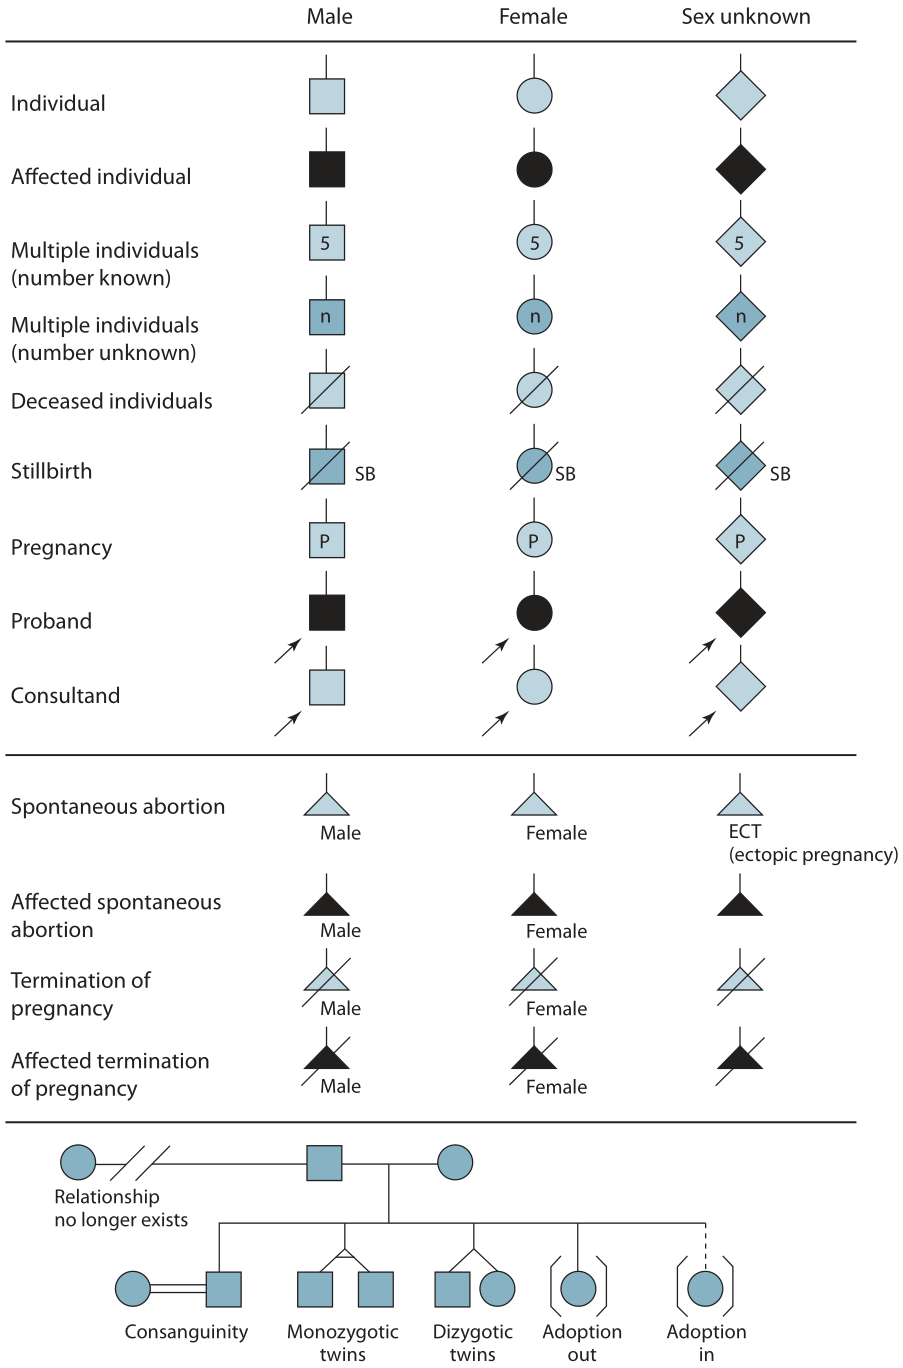
\includegraphics[scale=0.35]{images/pedigree.png}
\end{center}

\section{Inheritance Review}\label{Inhertiance Review}
\begin{itemize}
    \item \ddd{Psudodominant}: when a condition generated from an autosomal recessive trait that is common and compatible with reproduction.
      \begin{itemize}
        \item A ``false'' dominance, due to higher frequencies of homozygous carriers of the recessive allele.
      \end{itemize}
    \item \ddd{Penetrance}: the proportion of individuals carrying a particular variant that also express the trait.
      \begin{itemize}
        \item E.g., 60\% penetrance of autosomal dominant allele means 60\% of the population will express the trait to some degree.
      \end{itemize}
    \item \ddd{Expressivity}: the degree of phenotypic expression, not to be confused with penetrance. 
    \item \ddd{Allelic heterogeneity}: when different mutations at the same locus lead to the same or very similar phenotypes. 
    \item \ddd{Mosaicism}: when two or more populations of cells with different genotypes in one individual who has developed from a fertilized egg.
      \begin{itemize}
        \item Germline mosaicism occurs during gem cell development, which means mutations can be passed on despite not being present one generating the germline.
        \item Somatic mosaicism occurs when mutation occurs in early development, usually expressing mild or restricted manifestations of the phenotype. Only affects children if also present in germline.
      \end{itemize}
    \item \ddd{Trinucleotide repeat disorder}: a mutation in which repeats of three nucleotides increases until they cross a threshold above which they become unstable.
\end{itemize}


%\endgroup
%%%%%%%%%%% Patterns of Inheritance %%%%%%%%%%%
\end{document}